
Folgendes Beispiel zeigt, wie Absätze erfasst werden:

\begin{figure}[h!]
    \centering
      % 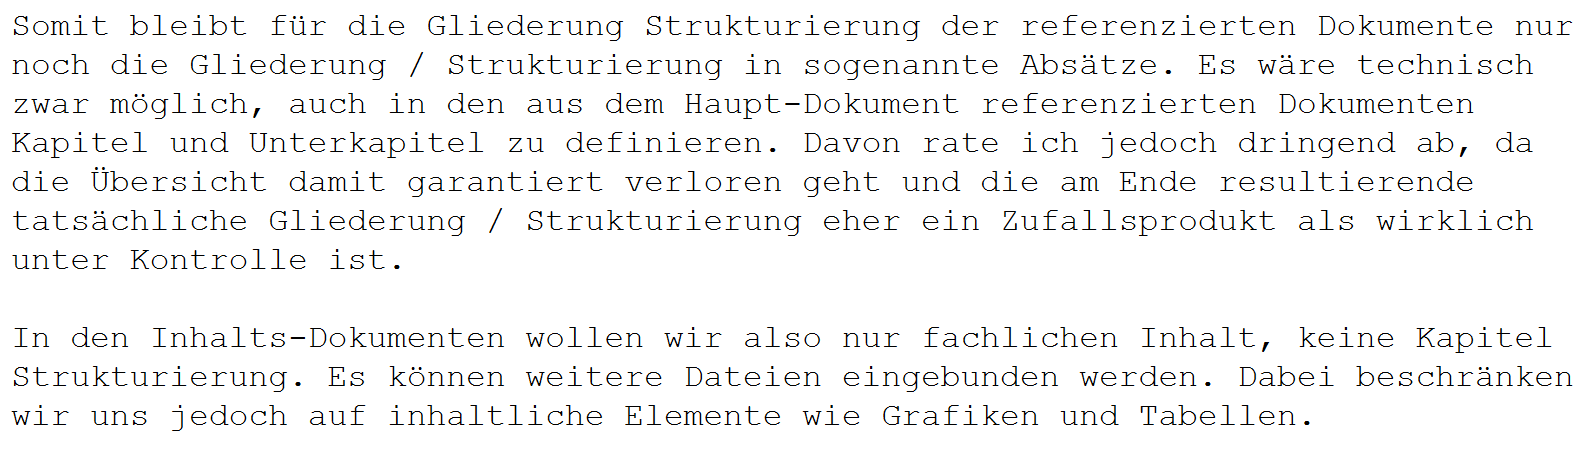
\includegraphics[width=0.85\textwidth]{./Bilder/GliederungAbsatz.png}        % Bild ohne Rahmen
      \fbox{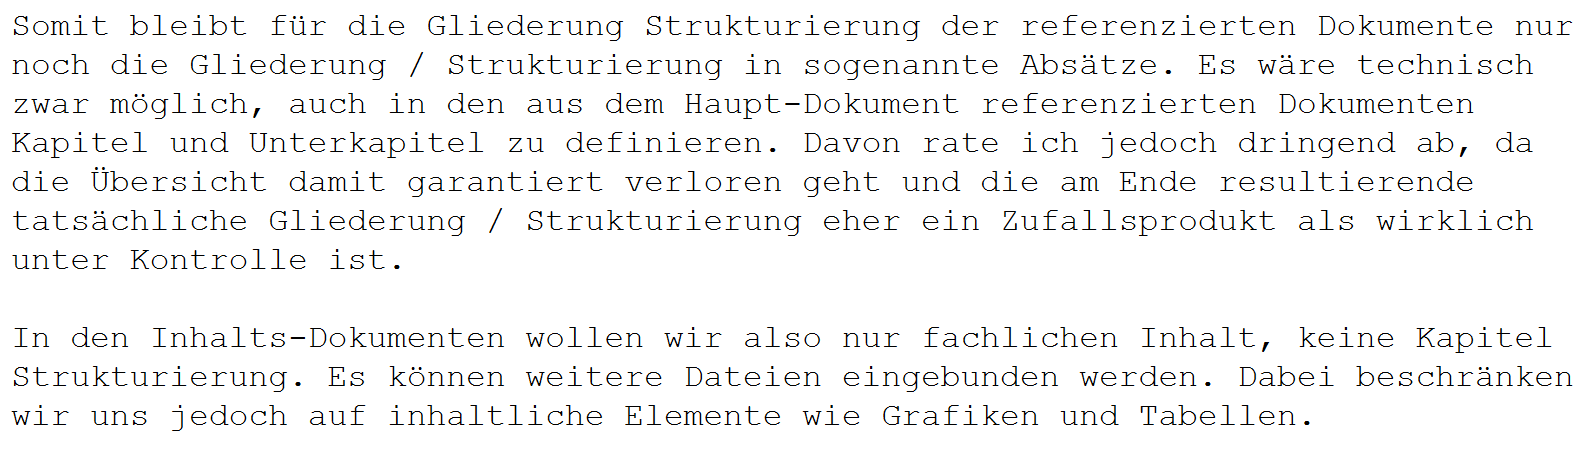
\includegraphics[width=0.85\textwidth]{./Bilder/GliederungAbsatz.png}}   % Bild mit Rahmen
      \caption{Absätze im Dokument}
    \label{fig:GliederungAbsatz}
\end{figure} 

Ein neuer Absatz wird durch eine Leerzeile im Text erzeugt. Die Anzahl der Leerzeilen und die Anzahl der Leerzeichen zwischen einzelnen Wörtern spielen keine Rolle. \LaTeX\ formatiert den (Fliess-) Text innerhalb eines Absatzes selber. Einfluss darauf wird über spezielle \LaTeX\ -Befehle genommen, die in folgenden Kapiteln behandelt werden.
 